\section{Background}
\label{sec:background}
Deep learning architectures are complex and a lot of research is going on. In the next sections we provide some basic background knowledge about recurrent neural network. If further background knowledge about neural networks is necessary, please read \cite{DeepLearning}.

\subsection{Recurrent Neural Network}
\label{sec:rnn}
There are many architectures specialized on different tasks. Convolutional networks are used for processing data that is organized as grid, like images. This kind of nets can also be used for time-series data, which are a 1-D grid. But often the data can not be interpreted as a 1-D grid and then another architecture is better suited. Recurrent neural networks (RNN) are specialized on processing sequential data.\\
\begin{figure}[thb]
	\caption{recurrent neural network with hidden-to-hidden connections \cite[p. 373]{DeepLearning}}
	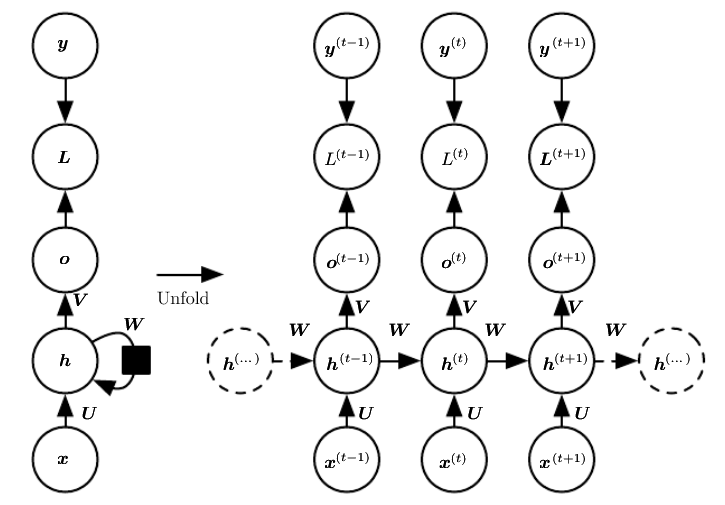
\includegraphics[width=0.95\linewidth]{images/rnn.PNG}
	\label{fig:rnn}
\end{figure}
The hidden units of a RNN have recurrent connections. So the result of a hidden unit at time step $t$ is used in the following time step $t+1$. It is important to notice that it is the same unit, which uses the result. As a consequence the parameters are shared during time. This is a key benefit, because it enables us to process sequences of different length. The update rule is also the same as it is the same unit.\\
There are different patterns, which combine the units in a different way. A RNN with connections between hidden units and a output at each time step (see figure \ref{fig:rnn}) can compute the same as a turing machine. In this sense the network is universal. It produces a sequence of outputs of the same length as the input. It is also possible to only produce a single output after the last hidden unit.\\
Like in any other neural network different output and loss functions are possible. Normally the softmax is used for the output. One common activation function is the hyperbolic tangent. The following equations show the update process of the forward propagation.
\begin{align}
a^{(t)} &= b + Wh^{(t-1)} + Ux^{(t)} \\
h^{(t)} &= tanh(a^{(t)}) \\
o^{(t)} &= c + Vh^{(t)} \\
y^{(t)} &= softmax(o^{(t)})
\end{align}
"where the parameters are the bias vectors b and c along with the weight matrices U, V and W, respectively, for input-to-hidden, hidden-to-output and hidden-to-hidden connections."\cite[p.374]{DeepLearning}\\
The generalized back-propagation algorithm can be applied to the unfolded computational graph. It is called back propagation through time (BPTT). You can see the unfold operation in figure \ref{fig:rnn}. Therefore, we need to store all the sequential states because they are used in the computation of the gradient. If we increase the number of recurrent layers the computational and memory cost increases as well. So for deep recurrent neural networks we have to meet the challenge of efficient training.

\subsection{Long-Term Dependencies}
\label{sec:ltd}
When we are training sequences of only length 10 to 20 the stochastic gradient descent (SGD) algorithm has already some problems. The gradients either tend to vanish, if it is in the interval $[0, 1[$, or tend to explode. The problem is that we reuse the unit in every time step and therefore the gradient is up to the power of the number of time steps.\\
Another problem is that the long-term dependencies have smaller magnitude on the weights than short-term dependencies have. The gradient is hidden by the smallest fluctuations arising from the short-term dependencies. As a consequence it takes very long time to train long-term dependencies. To overcome this problem we could introduce skipping connections where time step $t$ also uses the result from time step $t-2$ or even further in the past. So we have multiple time scales, one fine grained and one distant past.\\
Leaky units are a different way for remembering information about the past. A leaky unit is similar to a running average. A linear self-connection is used in the update rule.
\begin{align}
y^{(t)} = \alpha y^{(t-1)} + (1-\alpha)v^{(t)}
\end{align}
With the parameter $\alpha$ one could regulate how fast the information of the past is discarded. If $\alpha$ is near zero the information is kept for a long time. It would be the best if the network could learn this parameter and must not be set as a hyper parameter.

\subsection{Long Short-Term Memory}
\label{sec:lstm}
The Long Short-Term Memory (LSTM) is a gated recurrent neural network. Gated in this case means that the weight of the self-loop is controlled by another hidden unit. LTSM performed very good in handwriting and speech recognition, for example. The basic idea is that it might be useful to forget information of a leaky unit. As always it is better to have the network learn when to forget and not to decide manually.\\
\label{sec:lstm}
\begin{figure}[thb]
	\caption{long short-term memory cell \cite[p. 405]{DeepLearning}}
	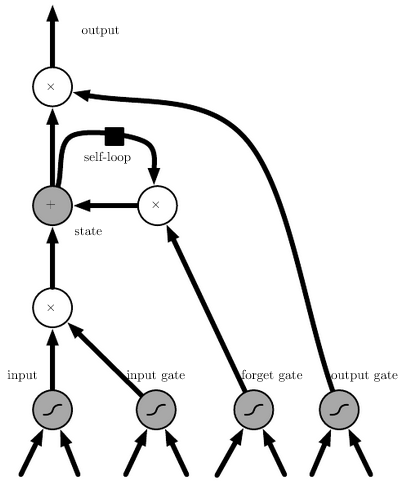
\includegraphics[width=0.95\linewidth]{images/lstmCell.PNG}
	\label{fig:lstm}
\end{figure}
In a LSTM network the hidden units consist of so called long short-term memory cells. A LSTM cell has three gating units (see figure \ref{fig:lstm}). The input gate is a sigmoid unit and controls the input feature. The input feature is a regular artificial neuron. The forget gate has the same task as the parameter $\alpha$ in a leaky unit. As there are only values between 0 and 1 are allowed, a sigmoid unit is used again. It controls how fast the information of the past is discarded. In other words it controls the weights of the state unit. The state unit has a self loop similar to the leaky units. With this self loop an internal recurrence is added to the outer recurrence of the LSTM cell. The output gate is also a sigmoid unit. It can shut off the output of the whole LSTM cell. So a Long Short-Term Memory network is far more complex than a simple recurrent neural network.

\subsection{Dropout}
\label{sec:dropout}

\subsection{k-Fold Cross Validation}
\label{sec:fcv}
